\documentclass[11pt]{article}

\usepackage[letterpaper,margin=1in]{geometry}
\usepackage[T1]{fontenc}
\usepackage{lmodern}
\usepackage{microtype}
\usepackage{amsmath,amssymb}
\usepackage{booktabs}
\usepackage{tabularx}
\usepackage{multirow}
\usepackage{graphicx}
\usepackage{xcolor}
\usepackage{upquote}
\usepackage{tikz}
\usetikzlibrary{arrows.meta,positioning,calc}
\usepackage[numbers,sort&compress]{natbib}
\usepackage[font=small,labelfont=bf]{caption}
\usepackage{enumitem}
\usepackage[colorlinks=true,linkcolor=oiblue,citecolor=oiblue,urlcolor=oiblue]{hyperref}
\usepackage{cleveref}

% Okabe--Ito palette, shared with the figures (make_figures.py)
\definecolor{oiblue}{HTML}{0072B2}
\definecolor{oiverm}{HTML}{D55E00}
\definecolor{oigreen}{HTML}{009E73}

\newcommand{\cg}{\textsc{ConceptGate}}
\newcommand{\raw}{\mathrm{raw}}
\newcommand{\LLR}{\mathrm{LLR}}

\setlist{itemsep=2pt,topsep=4pt}

\title{\cg: Few-Shot Concept Reading and Steering in Frozen Language Models}

\author{Nishan Pantha\\
Independent Researcher\\
\texttt{nishanpantha@gmail.com}}

\date{}

\begin{document}
\maketitle

\begin{abstract}
Deployed language models must detect and control concepts such as a jailbreak attempt, a topic, or a
tone. Often they have few examples and cannot retrain. One residual-stream
direction can detect a concept, and the same direction, added back, can steer generation. We test how far
this goes with about ten examples per class and closed-form fitting. \cg{} reads a concept at several
layers, fuses the layers with a learned depth filter, gates on a calibrated likelihood ratio, and steers
with a direction fit from the same examples. Against fair baselines on five models up to 2.6B parameters, most of the design fails. A logistic probe on the same layers matches the detector. Depth
fusion helps only on synthetic data. Mixture densities collapse to one component. A gate on concept
presence selects nothing, because it fires on 97\% of formatted attacks. One early result favoured the
gate, but it came from a missing chat template. With the template, the steering effect changed sign and
the gate's advantage disappeared. Three results survive. First, the few-shot direction is a refusal lever
in both directions (Qwen2.5-0.5B refusal: 64\% unsteered, 35\% steered away, 79\% steered toward). Second,
the gate's false-positive rate changes from 18\% to 96\% with the register of benign traffic. Third, on one
of two models, the unsteered activations predict a prompt's steerability (Spearman $\rho=0.58$,
permutation $z=6.7$). Steerability is how far a fixed write moves the prompt's sampled refusal rate. The
concept gate reads it at $|0.30|$, with the wrong sign. As a trigger, predicted steerability beats random
selection at every tested coverage. It does not replicate on gemma-2-2b, where more samples made the correlation fall. We also show how an unvalidated outcome measure gave a false null, and
why split-half reliability is not comparable across sample sizes.
\end{abstract}

% ===================================================================================================
\section{Introduction}
\label{sec:intro}

A frozen language model encodes many nameable properties of its input along approximately linear
directions in its residual stream~\citep{alain2016probes,zou2023repe,park2023linear}. A direction can be
read: this gives a probe. A direction can also be written back: this gives a steering
vector~\citep{turner2023actadd,panickssery2023caa}. This paper asks what we can build from these two facts
under tight constraints:
\begin{itemize}[leftmargin=*]
  \item no fine-tuning of the host model;
  \item about ten labelled examples per concept;
  \item closed-form fitting;
  \item kilobytes of storage per concept.
\end{itemize}

Our system, \cg{}, attaches to a frozen model. It does two things with one set of examples. It
\emph{detects} a concept from intermediate activations and returns a calibrated fire, abstain, or pass
decision. It \emph{steers} generation toward or away from the concept: it adds a related direction into
the residual stream. The first application was guardrails, but the mechanism is not specific to safety.
The concept is an input, given as data.

The design had two hypotheses:
\begin{enumerate}[leftmargin=*]
  \item \textbf{Read across depth.} A read over several layers is better than a read at the best single
    layer. If the layers carry independent evidence, a matched filter over depth combines them, and their
    discriminabilities add in quadrature.
  \item \textbf{Couple the read and the write.} If the write fires only where the read detects the concept,
    steering is more effective and causes less damage than steering on every prompt.
\end{enumerate}

Both hypotheses failed in the form we stated them. This paper reports each component against a fair
baseline. It shows which tests failed. It shows one strong result that came from an error in prompt
formatting. It also shows one positive result that came when we asked a different question of the same
system. We give the negative results the same weight as the positive results, because they contain most of
the useful information.

\paragraph{Summary of findings.}
\begin{enumerate}[leftmargin=*]
  \item \textbf{The read side gives no advantage over a probe.} A depth-matched logistic probe equals \cg{}
    at every tap (\cref{sec:detect}). Depth fusion gets its predicted gain on synthetic data that satisfies
    its assumption (test error 16.1\%$\to$9.4\%). It adds nothing on real models (\cref{sec:fusion}). The
    mixture density stays at one component (\cref{sec:mixture}). A training-free concept bank is
    30--38$\times$ cheaper to build than per-concept LoRA. A linear-probe bank has the same advantage
    (\cref{sec:bank}).
  \item \textbf{The write is a real lever, but not a new one.} Eight hand-written examples move generated
    refusal across a 43-point range, in either direction. On a first-token measure, the effect is about
    three times that of a matched-norm random direction (\cref{sec:write}). This is the refusal direction of
    \citet{arditi2024refusal}, recovered from few examples. It is not a new mechanism.
  \item \textbf{A gate on concept presence adds nothing. A gate on predicted effect helps, on one model.}
    On formatted attacks, the concept is almost always present, so the concept gate cannot select. A ridge
    read fit to the measured per-prompt effect of the write can select. On Qwen2.5-0.5B, it beats a
    size-matched random subset at every coverage. It does not replicate on gemma-2-2b (\cref{sec:dose}).
  \item \textbf{Three cautions on method.}
    \begin{enumerate}
      \item Prompt formatting alone reversed the sign of the main gate-steering effects. It also removed the
        apparent advantage of the gate (\cref{sec:formatting}).
      \item An outcome measure with unknown reliability can make a false null (\cref{sec:instrument}).
      \item Split-half reliability is not comparable across sample sizes (\cref{sec:splithalf}).
    \end{enumerate}
\end{enumerate}

No single mechanism here is new. Probes, difference-of-means directions, activation addition, Gaussian
density gates, and steering vectors conditioned on an activation read~\citep{lee2024cast,ferrando2025dsas}
all exist. Our contribution is the measurement. We map where a few-shot concept adapter works and where it
does not. We also give one possibly new result on per-prompt steerability.

% ===================================================================================================
\section{Related work}
\label{sec:related}

\paragraph{Probes and representation engineering.}
Linear probes read what a layer encodes linearly~\citep{alain2016probes}. Representation
engineering~\citep{zou2023repe} states that high-level concepts lie along directions that a user can read
and push. Its reading vectors come from PCA on paired activation differences. Our class-mean difference is
the construction of contrastive activation addition~\citep{panickssery2023caa}. Most such work uses one
layer, selected by a sweep. Our only change on the read side was to fuse several layers. It gave no gain
(\cref{sec:fusion}).

\paragraph{Activation steering and conditional steering.}
ActAdd~\citep{turner2023actadd} adds a contrastive direction to the residual stream. We use the form of
Contrastive Activation Addition~\citep{panickssery2023caa}. Circuit Breakers~\citep{zou2024circuitbreakers}
trains the model to reroute harmful representations. We steer a frozen model, so we accept less power for
less cost. CAST~\citep{lee2024cast} conditions a steering vector on an activation read. It applies or holds
a refusal vector based on a condition read from the prompt's hidden states. Thus the model refuses harmful
prompts and answers harmless prompts. DSAS~\citep{ferrando2025dsas} also separates when to steer from how
to steer. It scales the strength of an existing steering method per input and per layer. Thus the setting
of \cref{sec:write} is not new. Our contribution there is the controls. One direction mediates refusal~\citep{arditi2024refusal}. The model encodes harmfulness
separately from refusal~\citep{zhao2025harmfulness}. Steering along random or unrelated directions can
decrease refusal~\citep{korznikov2025roguescalpel,li2026pitfalls}. CAST's condition rules classify
mathematics problems as malicious and refuse them~\citep{sheng2025alphasteer}. Activation-trajectory
detectors for multi-turn attacks do not generalize equally across data sources~\citep{kulkarni2026lad}.
Our results agree with each of these observations. We get them from about ten examples.

\paragraph{Density-based detection.}
The Mahalanobis out-of-distribution detector~\citep{lee2018mahalanobis} scores with class-conditional
Gaussians. Our gate is a two-class case of it. Each class can optionally be a mixture, with the number of
components selected by BIC.

\paragraph{External classifiers and cost.}
The current standard for detection is a text classifier, such as Llama Guard~\citep{inan2023llamaguard},
or a fine-tuned multi-category guardrail on an encoder such as GLiNER~\citep{zaratiana2023gliner}. These
are strong. But they are a second model, and they can only read. To run only the layers below the deepest
tap is the detection equivalent of early exit~\citep{schuster2022calm}. Every latent probe gets this
saving. For the task of adding concepts to a model, the comparison is parameter-efficient
fine-tuning~\citep{houlsby2019adapters,hu2021lora}.

\paragraph{Predicting steering outcomes.}
\citet{fan2026asteer} train a classifier on ASTEER, their testbed of labelled steered generations. The
classifier predicts if an intervention will under-steer, succeed, or over-steer. Its features compare
hidden states before and after steering over the first decoding steps. \citet{billa2026where} uses a
logit-lens diagnostic to predict, per concept and per layer, if a difference-of-means steering vector will
be effective. \citet{ong2026sideeffects} use unsteered representations to predict the side effects of a
steering vector on other behaviours. Our first-token refusal-minus-compliance statistic is a basket-sum
variant of the refusal--affirmation logit gap of \citet{li2025logitgap}. The Cylindrical Representation
Hypothesis~\citep{gao2026crh} gives a geometric explanation of why steering sensitivity changes from sample
to sample. It does not predict the sensitivity from the unsteered prompt. We found no prior work that
predicts, from the unsteered prompt alone, how far a fixed write will move the behaviour on that prompt.

\paragraph{Adversarial limits.}
Obfuscated-activation attacks decrease the recall of latent-space probes to zero, and the target behaviour
continues~\citep{bailey2024obfuscated}. This limit applies to all results in this paper
(\cref{sec:limits}).

% ===================================================================================================
\section{Method}
\label{sec:method}

\begin{figure}[t]
\centering
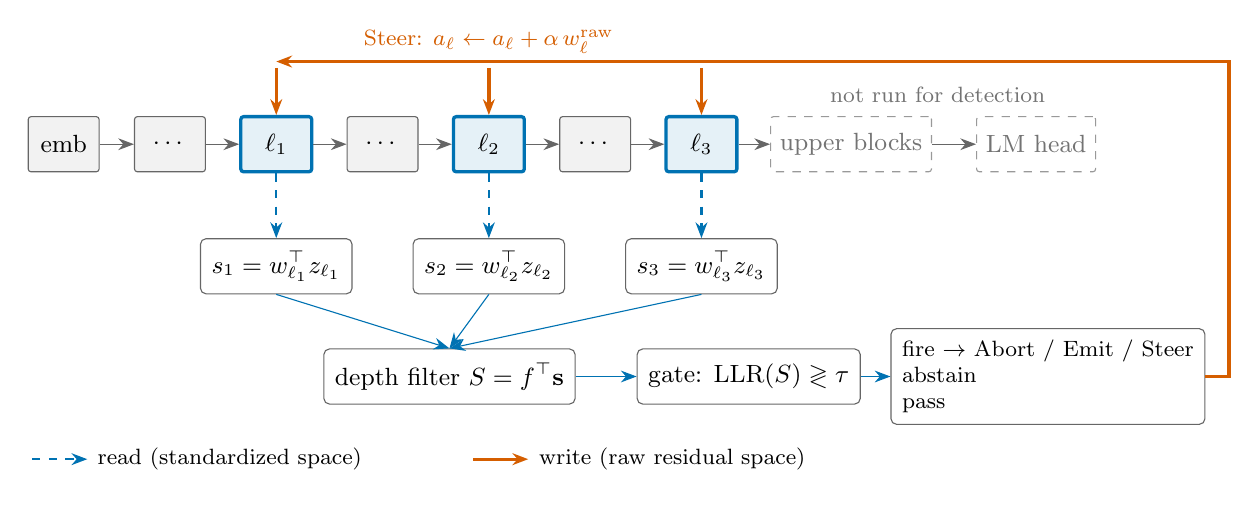
\begin{tikzpicture}[
  font=\small, >={Stealth[length=2mm]},
  blk/.style={draw=black!60, rounded corners=1pt, minimum width=9mm, minimum height=7mm, fill=black!5},
  tap/.style={blk, draw=oiblue, very thick, fill=oiblue!10},
  off/.style={blk, dashed, fill=none, text=black!55, draw=black!40},
  op/.style={draw=black!60, rounded corners=2pt, minimum height=7mm, inner sep=4pt, fill=white},
  rd/.style={->, oiblue, dashed, thick},
  wr/.style={->, oiverm, very thick},
]
\node[blk] (emb) at (0,0) {emb};
\node[blk] (b1) at (1.35,0) {$\cdots$};
\node[tap] (t1) at (2.7,0) {$\ell_1$};
\node[blk] (b2) at (4.05,0) {$\cdots$};
\node[tap] (t2) at (5.4,0) {$\ell_2$};
\node[blk] (b3) at (6.75,0) {$\cdots$};
\node[tap] (t3) at (8.1,0) {$\ell_3$};
\node[off, minimum width=19mm] (tail) at (10.0,0) {upper blocks};
\node[off] (head) at (12.35,0) {LM head};
\foreach \a/\b in {emb/b1,b1/t1,t1/b2,b2/t2,t2/b3,b3/t3,t3/tail,tail/head} \draw[->,black!60] (\a) -- (\b);
\node[anchor=south, black!55, font=\footnotesize] at (11.1,0.4) {not run for detection};

\foreach \i in {1,2,3} {
  \node[op] (s\i) at ($(t\i)+(0,-1.55)$) {$s_{\i} = w_{\ell_\i}^{\top} z_{\ell_\i}$};
  \draw[rd] (t\i) -- (s\i);
}
\node[op] (f) at (4.9,-2.95) {depth filter $S = f^{\top}\mathbf{s}$};
\foreach \i in {1,2,3} \draw[->,oiblue] (s\i.south) -- (f.north);
\node[op] (g) at (8.7,-2.95) {gate: $\LLR(S) \gtrless \tau$};
\draw[->,oiblue] (f) -- (g);
\node[op, align=left, font=\footnotesize, anchor=west] (act) at (10.5,-2.95) {fire $\to$ Abort / Emit / Steer\\abstain\\pass};
\draw[->,oiblue] (g) -- (act);

\draw[wr] (act.east) -- ++(0.3,0) |- (8.1,1.05) -- (2.7,1.05);
\foreach \i in {1,2,3} \draw[wr] ($(t\i.north)+(0,0.6)$) -- (t\i.north);
\node[oiverm, font=\footnotesize, fill=white, inner sep=1pt] at (5.4,1.3) {Steer: $a_\ell \leftarrow a_\ell + \alpha\, w^{\raw}_\ell$};

\draw[rd] (-0.4,-4.0) -- (0.3,-4.0) node[right, black, font=\footnotesize] {read (standardized space)};
\draw[wr] (5.2,-4.0) -- (5.9,-4.0) node[right, black, font=\footnotesize] {write (raw residual space)};
\end{tikzpicture}
\caption{The \cg{} pipeline. The frozen model runs up to the deepest tap. We standardize each tapped
activation and project it onto the concept direction of that layer. This gives one score per layer (the
\emph{spectrogram} $\mathbf{s}$). A depth filter combines the scores. A calibrated likelihood-ratio gate
returns fire, abstain, or pass. On a fire, an action can stop decoding, start a fixed continuation, or add
a raw-space direction back into the stream. The same examples fit this direction. The read and write
directions are related but not identical (per-tap cosine 0.45--0.83, \cref{sec:cosine}).}
\label{fig:pipeline}
\end{figure}

\Cref{fig:pipeline} shows the full path. All read-side fitting is closed form.

\subsection{Setup and standardization}
$M$ is a frozen causal language model with residual width $d$. We tap block outputs at layers
$\mathcal{L}=\{\ell_1,\dots,\ell_m\}$. Each prompt is represented by its \emph{last-token} activation
$a_\ell\in\mathbb{R}^d$. This token has attended to the full prompt. A fit on every token adds shared
boilerplate, which hides the signal. The positive and negative sets $\mathcal{A}^{\pm}$ each contain about
ten prompts. Residual streams have a few very large outlier dimensions. Thus, for detection, we standardize
per layer and per dimension with pooled statistics, $z=(a-\mu_0)\oslash(\sigma_0+\epsilon)$.

\subsection{Directions and the spectrogram}
The per-layer detection direction is the unit difference of the standardized class means:
\begin{equation}
w_\ell = \frac{\bar z^+_\ell - \bar z^-_\ell}{\lVert \bar z^+_\ell - \bar z^-_\ell\rVert}.
\end{equation}
In \emph{logistic} mode, it is a per-layer logistic-regression weight. Diff-of-means equals the LDA
direction $\Sigma^{-1}(\mu^+-\mu^-)$ only if the standardized dimensions are uncorrelated. Standardization
makes the marginal variances equal, but it does not remove correlations. The logistic mode closes this
gap. The projection at each layer, $s_\ell = w_\ell^\top z_\ell$, gives the profile of the concept across
depth. We call this profile the spectrogram $\mathbf{s}\in\mathbb{R}^m$.

\subsection{Depth filter and the quadrature argument}
\label{sec:quadrature}
A filter $f\in\mathbb{R}^m$ reduces the spectrogram to one score, $S=f^\top\mathbf{s}$. We use three
filters:
\begin{itemize}[leftmargin=*]
  \item \texttt{best}: a one-hot on the most discriminative layer. This is the single-layer baseline.
  \item \texttt{diag}: each layer has a weight equal to its own signal-to-noise ratio.
  \item \texttt{fisher}: $f\propto\Sigma_{\mathbf{s}}^{-1}(\bar{\mathbf{s}}^+-\bar{\mathbf{s}}^-)$, with a
    ridge-regularized pooled covariance.
\end{itemize}
\texttt{best} is a nested special case. Thus a comparison of the filters isolates the effect of depth.

The motivation is a matched-filter argument. Let $s_\ell = a_\ell y + n_\ell$, with $y\in\{\pm1\}$ and
independent noise $n_\ell\sim\mathcal{N}(0,\sigma_\ell^2)$. Then the filter $f_\ell\propto
a_\ell/\sigma_\ell^2$ gives the maximum discriminability after the combination, and
\begin{equation}
d'_{\text{comb}} = \Big(\sum_\ell {d'_\ell}^2\Big)^{1/2} \ \ge\ \max_\ell d'_\ell ,
\end{equation}
with equal-prior error $\Phi(-d'/2)$. The critical assumption is independence across layers. Adjacent
residual-stream layers are not independent. This is why the argument fails in practice (\cref{sec:fusion}).

\subsection{Calibrated gate and mixtures}
We fit class-conditional densities to the score. The gate fires when $\LLR = \log p(\cdot\mid +) - \log
p(\cdot\mid -) > \tau$. We set the threshold on the benign tail. Two rules are available: a false-positive
quantile, or the point $z$ standard deviations above the benign mean ($z=3$ is approximately a 0.1\%
tail). We map the LLR to $P_{\text{present}}=\sigma((\LLR-\tau)/s)$, where $s$ is the benign spread near
$\tau$. The gate abstains when $|P_{\text{present}}-\tfrac12|$ is less than a margin. As an option, each
class is a Gaussian mixture on the joint spectrogram, with $J\in\{1,2,3\}$ components selected by BIC.
With $J=1$ and a shared covariance, the LLR is affine in $\mathbf{s}$. It then reduces exactly to the
\texttt{fisher} filter.

A bank of $K$ concepts fires if one or more concepts fire. It assigns the fire to the concept with the
largest LLR. Per-concept thresholds do not compose. An OR over $K=14$ concepts at $z=3$ gives a bank-level
false-positive rate of up to approximately 1.4\%. Thus the operating point must be set for the full bank.

\subsection{Steering}
\label{sec:steering}
The steering hook sees raw activations. Thus the write uses a separate raw-space direction per tap,
$w^\raw_\ell = (\bar a^+_\ell - \bar a^-_\ell)/\lVert \bar a^+_\ell - \bar a^-_\ell\rVert$. During
generation, the hook applies $a_\ell \leftarrow a_\ell + \alpha\, w^\raw_\ell$. A positive $\alpha$ steers
toward the concept. A negative $\alpha$ steers away from it. The residual norm of GPT-2 is approximately
five times that of Qwen2.5-0.5B (96 and 18 in our runs). Thus we set $\alpha$ as a fraction of the
measured residual norm. In development runs, 3--10\% kept the text coherent. Above approximately 20--25\%,
the text became repetitive.

\subsection{Actions, triggers, and the truncated forward}
Detection and steering use one interface. An action (\texttt{Abort}, \texttt{Emit}, \texttt{Steer}) runs
when its trigger is true. The triggers are \texttt{FIRE}, \texttt{FIRE\_OR\_UNSURE}, and \texttt{ALWAYS}.
We added two triggers after the work in \cref{sec:dose}. \texttt{Predicted(name, $\tau$)} fires on the
prediction of an outcome head, not on concept membership. \texttt{Both(a, b)} requires both conditions.
Detection needs only blocks $0..\max\mathcal{L}$. On GPT-2, the truncated forward is bit-identical at the
taps and 1.75$\times$ faster than a full forward. A weight-truncated load mode never loads the upper
blocks. Generation still needs the full model. \Cref{app:api} lists the library calls.

\subsection{Cost}
\Cref{tab:storage} lists what one concept stores. For GPT-2 with five taps, the total is approximately
$1.5\times10^4$ numbers. For the three-tap configurations below, it is 11--28 thousand. A fit is a few
means and one $m\times m$ solve. It takes milliseconds on a CPU.

\begin{table}[h]
\centering
\small
\caption{Storage per concept ($m$ taps, residual width $d$).}
\label{tab:storage}
\begin{tabular}{lc}
\toprule
Item & Numbers \\
\midrule
read and write direction sets & $2md$ \\
standardization statistics & $2md$ \\
depth filter & $m$ \\
gate & a few scalars \\
\bottomrule
\end{tabular}
\end{table}

% ===================================================================================================
\section{Experimental setup}
\label{sec:setup}

\paragraph{Models.} GPT-2 (12 blocks, float32), Qwen2.5-0.5B-Instruct (24 blocks), and gemma-2-2b-it (26
blocks). One sweep also uses SmolLM2-360M-Instruct and SmolLM2-1.7B-Instruct. Instruct models load in
bfloat16 unless stated. The first GPT-2 and Qwen detection results ran on a CPU. All other runs used an
Apple M4 GPU (MPS).

\paragraph{Data.} \Cref{tab:data} lists the data for each experiment.

\begin{table}[h]
\centering
\small
\caption{Data per experiment.}
\label{tab:data}
\begin{tabularx}{\textwidth}{>{\raggedright\arraybackslash}p{3.2cm}>{\raggedright\arraybackslash}X}
\toprule
Experiment & Data \\
\midrule
Jailbreak detection & \texttt{jackhhao/jailbreak-classification}~\citep{jackhhao2023jailbreak}. Fit on the
  training split. Scored on the official test split (262 prompts: 139 jailbreak, 123 benign). \\
Multi-concept bank & The fourteen harm categories of BeaverTails~\citep{ji2023beavertails}. Positives are
  prompts whose responses have that annotation. Negatives come from a shared benign pool. \\
Topical steering & Hand-written few-shot sets for \emph{food}, \emph{nature}, and \emph{technology}. \\
Steering gate (\cref{sec:write,sec:dose}) & Hand-written short override framings; held-out jailbreak
  templates with a harmful request appended; bare harmful requests; real benign prompts. \\
\bottomrule
\end{tabularx}
\end{table}

\paragraph{Prompt formatting.} Detection benchmarks read raw prompts. From \cref{sec:formatting} onward,
all steering and gate experiments format prompts with the chat template of the model, for reading and for
generation. \Cref{sec:formatting} explains why this is important.

\paragraph{Statistics.} Unless stated, $\pm$ is the standard deviation over three few-shot resamples.
Correlations are Spearman. Permutation nulls run the identical pipeline again on shuffled targets.

% ===================================================================================================
\section{The read side: a sequence of negative results}
\label{sec:read}

\subsection{Depth fusion works only where its assumption holds}
\label{sec:fusion}
The synthetic data has three independent layers with known $d'=[1.6, 2.0, 0.6]$. Theory predicts a fused
$d'=2.63$ and a test error of $\Phi(-1.315)=9.4\%$. The best single layer gives $\Phi(-1.0)=15.9\%$. The
learned filter recovers $d'=[1.62,2.04,0.64]$. It decreases the test error from 16.1\% to 9.4\%. This
result shows only that the code implements the algebra correctly. We generated the data under the
assumption of the filter, so the result is almost a tautology.

On real models, the gain disappears (\cref{fig:depth}, \cref{tab:detect}). Three-tap and five-tap fusions
are equal to the best single tap. On Qwen2.5-0.5B, a logistic probe on the concatenated taps is slightly
better than the \cg{} fusion (0.978 and 0.973). The tapped layers are too correlated for quadrature to
apply.

\subsection{Mixture densities collapse}
\label{sec:mixture}
Mixtures can be important. We made a test case with benign clusters on the two sides of the harmful
cluster. No linear threshold works on it (38.8\% error, AUC 0.60). A two-component mixture gets 7.1\%
error (AUC 0.98; the Bayes floor is 5.8\%). We made this case directly in score space. Its class means are
the same, so our direction-finding cannot make it from real data.

On real GPT-2 activations with 12 prompts per class, BIC selects $J=1$ for both classes. On held-out
prompts, the mixture gate and the single-Gaussian gate agree at a rank correlation of 0.986. Sample size is
not the only cause (\cref{tab:bic}). On the jailbreak benchmark, in diff-of-means mode, BIC selects one
component per class up to 64 examples per class on both models. This is far past the point where a
three-dimensional covariance is estimable. When BIC selects a second component, the held-out AUC gain is
0.007 or less.

\begin{table}[t]
\centering
\small
\caption{Components selected by BIC (positive / negative class, median of three seeds) as the fit size
$N$ per class increases. Three taps at 33/50/67\% depth. The last row is the largest held-out AUC gain of
the BIC-selected gate over the same gate with $J=1$, across both models and both modes.}
\label{tab:bic}
\begin{tabular}{lccccc}
\toprule
$N$ per class & 12 & 32 & 64 & 128 & 256 \\
\midrule
Qwen2.5-0.5B, diff-of-means & 1/1 & 1/1 & 1/1 & 1/\textbf{2} & \textbf{2}/\textbf{2} \\
Qwen2.5-0.5B, logistic & 1/1 & 1/1 & 1/1 & \textbf{2}/\textbf{2} & \textbf{2}/\textbf{2} \\
gemma-2-2b, diff-of-means & 1/1 & 1/1 & 1/1 & 1/1 & \textbf{2}/\textbf{2} \\
gemma-2-2b, logistic & 1/1 & 1/1 & \textbf{2}/1 & \textbf{2}/\textbf{2} & \textbf{2}/\textbf{2} \\
\midrule
best held-out AUC gain & 0.000 & 0.000 & +0.001 & +0.006 & +0.007 \\
\bottomrule
\end{tabular}
\end{table}

\subsection{Matched negatives hurt, and a predicted robustness effect is absent}
\label{sec:negatives}
CAA~\citep{panickssery2023caa} suggests that benign negatives in the same surface register as the
jailbreaks make the direction more precise. We expected this result. On the development set (15 negatives
of each type), matched negatives gave AUC 0.42. Broad negatives gave 0.78. At this sample size, we read
0.42 as a failure to separate, not as a stable inversion. Broad negatives let the direction align with the
large semantic gap between an instruction to the model and an ordinary query. Matched negatives remove
this gap.

We also expected that paraphrase would break shallow taps but not deep taps. That result would give a
reason to tap deep. But rewording the positives has almost no effect on AUC at any layer. Against broad
negatives, detection uses the same semantic gap, and rewording does not close it.

\subsection{Detection gives no advantage over a probe}
\label{sec:detect}
At each single tap, the \cg{} logistic direction and a depth-matched logistic probe give the same number.
The reason is that a single-tap logistic direction is logistic regression on that tap. Thus the fair
single-concept comparison is a tie. The only gap is to a probe on the final layer, which runs the full
model (\cref{tab:detect}). At three taps, diff-of-means is 2--5 AUC points below logistic. Thus every
comparison with a trained classifier uses logistic mode. \Cref{fig:nshot} shows the same pattern on four
models, at every sample size from four to 32 examples per class. Logistic regression on the same taps
equals \cg{}-logistic from 16 examples per class. Below 16, it is equal or better.

\begin{figure}[t]
\centering
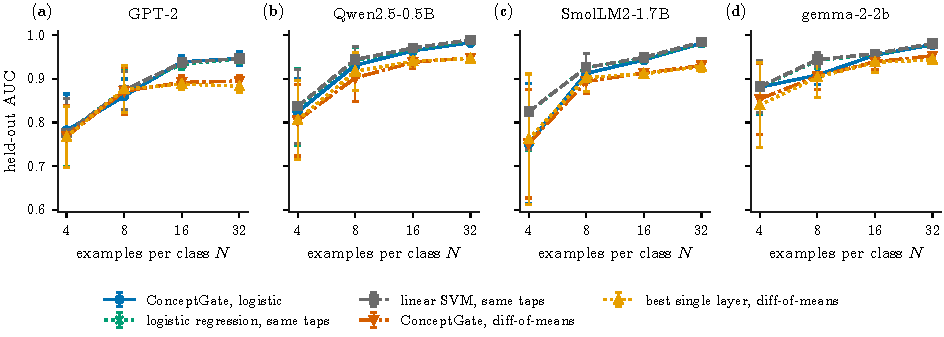
\includegraphics[width=\textwidth]{figures/fig_nshot.pdf}
\caption{Sample efficiency on jailbreak detection: held-out AUC as the number of examples per class
increases. Every method reads the same three tapped activations (mean $\pm$ s.d. over three resamples).
Logistic regression on the taps is within 0.006 of \cg{}-logistic at $N\geq16$. At $N\leq8$, where the
resample spread is large, it is better by up to 0.07. Diff-of-means fusion is within $\pm0.015$ of the best
single layer at all $N$. This run is separate from \cref{tab:detect} and has its own resamples. Thus the
values at $N=32$ differ from that table by up to 0.01.}
\label{fig:nshot}
\end{figure}

\begin{figure}[t]
\centering
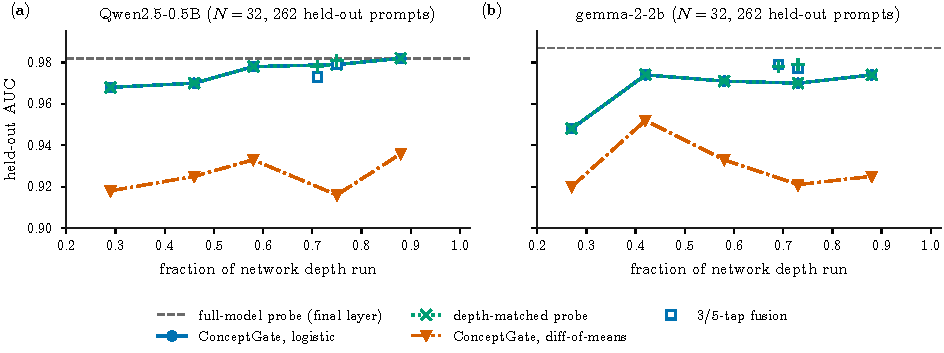
\includegraphics[width=\textwidth]{figures/fig_depth.pdf}
\caption{Held-out jailbreak-detection AUC against the fraction of network depth that runs ($N=32$ per
class, three resamples). Filled markers are single taps. Hollow squares are three-tap and five-tap fusions.
Plus signs are the depth-matched probe on the same taps. \cg{}-logistic and the depth-matched probe are
equal at every single tap. Fusion adds nothing over the best single tap. The gap to the dashed line is the
cost of a partial network. It is not an advantage of one method.}
\label{fig:depth}
\end{figure}

\begin{table}[t]
\centering
\small
\caption{Single-concept jailbreak detection, $N=32$ per class, 262 held-out prompts. Depth and weights are
the fractions of the network that runs and that loads. They are exact properties of the truncation. We do
not give wall-clock ratios, because they changed by several points between runs.}
\label{tab:detect}
\begin{tabular}{llccc}
\toprule
Model & Configuration & AUC & Depth & Weights \\
\midrule
\multirow{6}{*}{Qwen2.5-0.5B}
 & \cg{} logistic, 1 tap (L10) & $0.970\pm0.011$ & 46\% & 61\% \\
 & depth-matched probe, 1 tap (L10) & $0.970\pm0.011$ & 46\% & 61\% \\
 & \cg{} logistic, 3 taps (L8/12/16) & $0.973\pm0.009$ & 71\% & 79\% \\
 & depth-matched probe, 3 taps & $0.978\pm0.010$ & 71\% & 79\% \\
 & \cg{} diff-of-means, 3 taps & $0.927\pm0.017$ & 71\% & 79\% \\
 & full-model probe (final layer) & $0.982\pm0.003$ & 100\% & 100\% \\
\midrule
\multirow{6}{*}{gemma-2-2b}
 & \cg{} logistic, 1 tap (L10) & $0.974\pm0.010$ & 42\% & 55\% \\
 & depth-matched probe, 1 tap (L10) & $0.974\pm0.010$ & 42\% & 55\% \\
 & \cg{} logistic, 3 taps (L9/13/17) & $0.979\pm0.008$ & 69\% & 76\% \\
 & depth-matched probe, 3 taps & $0.978\pm0.007$ & 69\% & 76\% \\
 & \cg{} diff-of-means, 3 taps & $0.958\pm0.017$ & 69\% & 76\% \\
 & full-model probe (final layer) & $0.987\pm0.003$ & 100\% & 100\% \\
\bottomrule
\end{tabular}
\end{table}

The truncated forward is a real saving over the full-model probe. On Qwen2.5-0.5B, one tap at 46\% depth
gets 0.970 and loads 61\% of the weights. Every latent probe gets this saving. Thus it shows how early the
model forms the concept. It is not a property of \cg{}.

A leave-one-out layer sweep on about 20 prompts found the jailbreak concept separable at block 1 of 24 on
Qwen2.5-0.5B. On GPT-2, it was separable only at approximately block 6 of 12. To select the knee on the same
small estimate biases it upward. Thus the 262-prompt numbers above are the reliable values. The comparison also
has a confound: Qwen2.5 is instruction-tuned on refusal, and GPT-2 is a 2019 base model.

\paragraph{A first generalization test with a confound.} Our first cross-distribution test trained on one
dataset and tested on the other (jailbreak framing and BeaverTails harmful content). \cg{} and a probe
both fell to approximately chance (AUC 0.36--0.52). These are two different concepts. Thus the test
measured concept transfer, which fails for all methods. It did not measure robustness. \Cref{sec:ood}
replaces it with a within-concept test.

\subsection{A concept bank: cheaper than fine-tuning, equal to a probe bank}
\label{sec:bank}
\Cref{tab:bank} compares three ways to add the fourteen BeaverTails categories at $N=32$. In \cg{}, a
concept is a closed-form fit. A rank-8 LoRA adapter with a classification head must train. The full
fourteen-category bank takes approximately 8\,s on Qwen2.5-0.5B and 46\,s on gemma-2-2b. LoRA takes 3.9
and 29 minutes (30$\times$ and 38$\times$). One truncated forward serves all concepts. Thus inference cost
does not change with $K$. $K$ LoRA adapters need $K$ forwards. Detection quality stays high. We also ran
few-shot LoRA on three categories. It gets mean AUC 0.685 (Qwen) and 0.814 (gemma). \cg{} gets 0.889 and
0.913 on the same three.

\begin{table}[t]
\centering
\footnotesize\setlength{\tabcolsep}{4pt}
\caption{Per-concept cost and mean detection AUC over fourteen BeaverTails categories ($N=32$, three
seeds). In the last row, the probe heads read the \cg{} taps, not the final layer. The cost is the same.}
\label{tab:bank}
\begin{tabular}{lccc}
\toprule
 & \cg{} & linear probe & LoRA (rank 8) \\
\midrule
learn, Qwen2.5-0.5B / gemma-2-2b & 6 / 11 ms & 2 / 2 ms & 16.7 / 125.8 s \\
parameters per concept & 11--28 K & 0.9--2.3 K & 0.54--1.6 M \\
inference over $K$ concepts & one shared forward & one shared forward & one forward each \\
mean AUC, Qwen / gemma & 0.832 / 0.881 & 0.855 / 0.874 & --- \\
probe heads at \cg{}'s taps & --- & 0.840 / 0.880 & --- \\
\bottomrule
\end{tabular}
\end{table}

A linear-probe bank has all of these advantages. The first comparison in the table gave the probe a depth
advantage: its heads read the final layer, and \cg{} read three taps up to 91\% of the backbone. We fit the
same heads again on the \cg{} taps from cached activations. They get 0.840 on Qwen and 0.880 on gemma. On
gemma this is a tie (the probe is better on 8 of 14 categories). On Qwen the probe has a small advantage
(better on 10 of 14). \cg{} adds one thing: a write direction per concept, with no extra fit cost. For
these harm categories, this direction points the wrong way (\cref{sec:harmbank}).

Two cautions apply to the labels:
\begin{itemize}[leftmargin=*]
  \item BeaverTails annotates responses. Thus a response-level label replaces a prompt-level concept.
  \item One shared benign pool pulls all fourteen directions toward a common centroid. Thus the bank is
    nearer to one harmfulness direction with category-specific variation than to fourteen independent
    concepts.
\end{itemize}

\subsection{Held-out harm categories}
\label{sec:ood}
This test measures generalization within one concept. We hold out one category at a time. We fit on the
other thirteen plus the shared benign pool, and we score the held-out category. The comparison is a
direction fit on the held-out category itself (\cref{fig:ood}). \Cref{tab:oodsummary} gives the mean AUC.
Generalization is partial. Violence, self-harm, drugs and weapons, terrorism, and financial crime stay
detectable (0.74--0.78 on Qwen, 0.67--0.75 on gemma). Controversial politics (0.39--0.47) falls to chance
or below. On gemma, sexual content (0.43) also falls below chance.

\begin{table}[h]
\centering
\small
\caption{Mean AUC over fourteen BeaverTails categories, fit on the category itself and with the category
held out.}
\label{tab:oodsummary}
\begin{tabular}{llcc}
\toprule
Model & Method & In-distribution & Held out \\
\midrule
\multirow{2}{*}{Qwen2.5-0.5B} & \cg{} & 0.827 & 0.647 \\
 & probe & 0.847 & 0.610 \\
\midrule
\multirow{2}{*}{gemma-2-2b} & \cg{} & 0.868 & 0.616 \\
 & probe & 0.866 & 0.610 \\
\bottomrule
\end{tabular}
\end{table}

On Qwen, the held-out AUC of \cg{} is better than that of the probe in 13 of 14 categories, by
$0.037\pm0.032$ (s.d. across categories). On gemma, the two are equal (7 of 14, $0.007\pm0.028$). We give no
$p$-value for 13 of 14. The leave-one-out fit sets overlap, so the categories are not independent trials.

\begin{figure}[t]
\centering
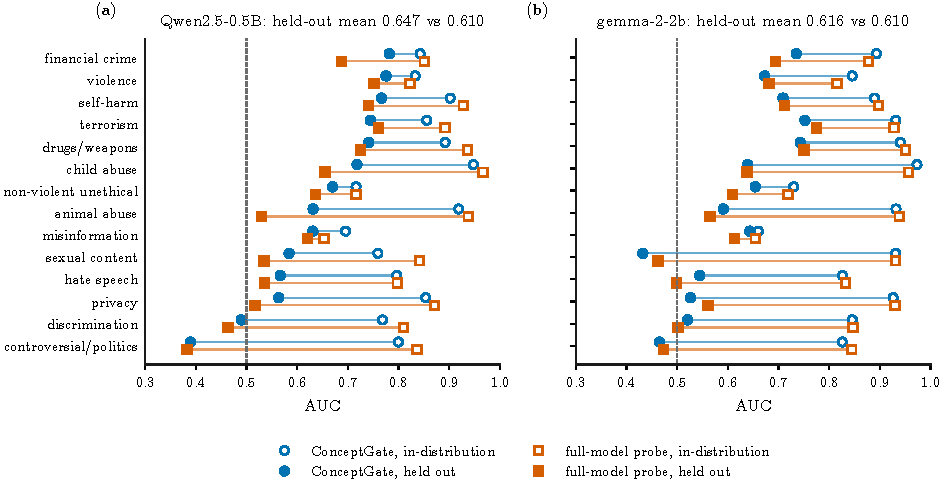
\includegraphics[width=\textwidth]{figures/fig_ood.pdf}
\caption{Leave-one-category-out generalization over fourteen BeaverTails categories. Hollow markers:
direction fit on the evaluated category (in-distribution). Filled markers: direction fit on the other
thirteen (held out). The line between them is the decrease. Categories are in order of the \cg{} held-out
AUC on Qwen2.5-0.5B. The dashed line is chance.}
\label{fig:ood}
\end{figure}

% ===================================================================================================
\section{The write side}
\label{sec:write}

\subsection{Dose-response on topical concepts}
\label{sec:topical}
For \emph{food}, \emph{nature}, and \emph{technology}, we steer greedy continuations of five neutral
prompts across $\alpha\in[-0.16,0.16]$. We score each continuation in three ways:
\begin{itemize}[leftmargin=*]
  \item the share of content words in a hand-written concept keyword list;
  \item perplexity under the base model;
  \item the LLR of the concept's own detector on the generated text.
\end{itemize}
The keyword list is not part of the fit. But the same author wrote the list and the few-shot prompts, so
their framing is not independent. There is no baseline method: a probe cannot steer, and the rule itself is
activation addition. The comparisons are the unsteered point and the two models.

\begin{figure}[t]
\centering
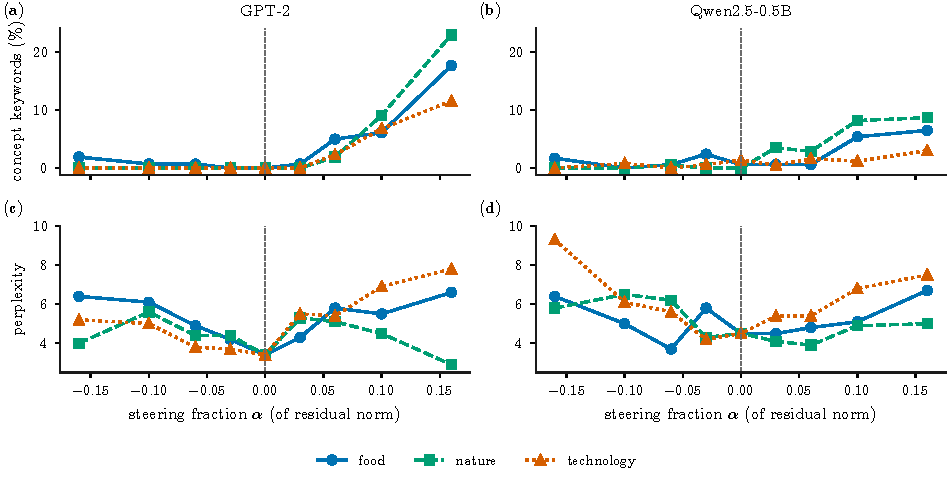
\includegraphics[width=\textwidth]{figures/fig_steer.pdf}
\caption{Steering dose-response on topical concepts: concept keyword rate (top) and perplexity (bottom)
of greedy 40-token continuations of five neutral prompts, against the steering fraction $\alpha$. On
Qwen2.5-0.5B, content increases with $\alpha>0$, and perplexity stays approximately flat up to
$|\alpha|\approx0.1$. GPT-2 moves content further, but as degenerate repetition. On Qwen, technology, the
most abstract concept, moves least.}
\label{fig:steer}
\end{figure}

On Qwen2.5-0.5B, content increases with $\alpha$ toward the concept. Perplexity stays approximately flat up
to $|\alpha|\approx0.1$ (\cref{fig:steer}). The LLR of the concept's own detector increases over the food
sweep, with one reversal between adjacent steps. The nature LLR changes from negative to positive. At large
$\alpha$, GPT-2 moves content further (23\% nature keywords, against 9\% on Qwen). But the text is
repetition (``the sun shone on the mountains, and the moon shone on the mountains\ldots''). The GPT-2
detector almost does not see the change: the nature LLR stays negative at all $\alpha$. Abstract concepts
move least. \Cref{tab:examples} shows the continuations for one prompt.

\begin{table}[t]
\centering
\footnotesize
\caption{Greedy continuations of ``The best part of the day was when'' under steering (first
${\sim}130$ characters). All concepts share the same unsteered continuation.}
\label{tab:examples}
\begin{tabularx}{\textwidth}{llX}
\toprule
Model & Write & Continuation \\
\midrule
\multirow{3}{*}{Qwen2.5-0.5B}
 & none & I got to see my friend's family. It was a nice surprise, and it made me feel happy. A. surprised B. excited C.\ldots \\
 & nature, $+0.10$ & I saw a group of people in the park. The sun was shining and the birds were singing. It was peaceful, like nothing else.\ldots \\
 & food, $+0.16$ & you get to make your own food. I love making homemade salsa, and this is a great way to use up some of the veggies\ldots \\
\midrule
\multirow{3}{*}{GPT-2}
 & none & I got to the airport and I was greeted by a guy who was a little older than me. He was a guy who was a little\ldots \\
 & nature, $+0.10$ & the sun was shining through the trees and the trees were covered with the leaves of the trees. The sun was shining\ldots \\
 & nature, $+0.16$ & the sun shone on the mountains, and the moon shone on the mountains, and the moon shone on the mountains\ldots \\
\bottomrule
\end{tabularx}
\end{table}

\subsection{Is GPT-2's weak self-read a geometric artifact?}
\label{sec:cosine}
The read and write directions are different. We map the detection direction to raw space and compare it
with the raw steering direction. Their mean $|\cos|$ is between 0.45 and 0.83. The value changes with the
model, the concept, and the mode (\cref{tab:cosine}). Chance is approximately $1/\sqrt d$ (0.021--0.036),
so the two directions are related. But they are 34--63 degrees apart, so they are not the same vector.
Logistic mode always gives a lower value. By design, it rotates away from the class-mean difference.

\begin{table}[t]
\centering
\small
\caption{Mean $|\cos|$ between the read direction (mapped to raw space) and the write direction, over
three taps and four concepts, on raw prompts.}
\label{tab:cosine}
\begin{tabular}{lccc}
\toprule
 & GPT-2 ($d$=768) & Qwen2.5-0.5B ($d$=896) & gemma-2-2b ($d$=2304) \\
\midrule
diff-of-means detection & $0.79\pm0.06$ & $0.65\pm0.07$ & $0.75\pm0.07$ \\
logistic detection & $0.68\pm0.11$ & $0.59\pm0.09$ & $0.71\pm0.09$ \\
logistic, jailbreak (32 real/class) & 0.52 & 0.45 & 0.57 \\
\bottomrule
\end{tabular}
\end{table}

This gap gives a possible second explanation for the weak self-read on GPT-2: the write moves activations
to a place where the read does not look. We tested this directly. We steered, read the continuation again,
and projected it onto the two directions. On GPT-2, the steered output also moves along the detection
direction: by $+4.2$ and $+2.1$ standardized units at two of three taps. The total LLR change is $+21$. On
Qwen, the change is $+48$. Also, GPT-2 is not the least-aligned model in any mode. Qwen is, and the Qwen
read follows its write well. Thus the geometric explanation is wrong. The GPT-2 read stays negative because
the concept is poorly separated in that model.

\subsection{Gate-conditioned steering, first attempt: a result that reversed}
\label{sec:formatting}
The steering rule is activation addition. Thus the read side can contribute to the write in only one way:
it can decide \emph{when} to write. Our first measurement of this looked like a clear win.

\paragraph{Design.} Qwen2.5-0.5B-Instruct, taps 8/12/16. We fit a jailbreak concept in logistic mode from
eight hand-written override framings and eight short benign requests, over three resamples. We calibrate
at $z=2$. The test set has 32 held-out framed attacks, 32 in-register benign requests, and 32 real benign
prompts from the held-out split of the dataset. We use the real benign prompts only to measure
out-of-register fires. The write magnitude is $\alpha=0.08$. \Cref{tab:arms} lists the arms. Refusal is the
share of continuations that match an explicit-decline lexicon. Collateral damage is perplexity and the
share of benign continuations that stay byte-identical.

\begin{table}[h]
\centering
\small
\caption{Arms of the gate experiment.}
\label{tab:arms}
\begin{tabularx}{\textwidth}{l>{\raggedright\arraybackslash}X}
\toprule
Arm & Prompts that get the write \\
\midrule
no steer & none \\
always & all \\
gated & prompts where the gate fires \\
random & a random subset of the same size as the gated set, matched within attacks and within benign prompts \\
anti-gate & prompts where the gate passes \\
sign-flipped & the same prompts as one of the arms above, with the opposite sign of $\alpha$ \\
\bottomrule
\end{tabularx}
\end{table}

\paragraph{The first result.} With no chat template, the gate fired on 54\% of attacks and 10\% of
in-register benign prompts. On the gated prompts, steering away from the concept increased refusal from
46.9\% by $+8.3\pm1.5$ points. A random subset of the same size gained only $+1.0\pm3.9$. The anti-gate arm
\emph{lost} $6.2\pm2.6$. The sign-flip arms seemed to explain this. On prompts where the gate fired, the two
signs moved refusal in opposite directions, so the direction looked like a lever. On prompts where the gate
passed, both signs decreased refusal, so the write looked like noise. The interpretation was ``selection,
not dosage'': the gate finds the prompts on which the write has a meaning.

\paragraph{The audit.} A read of the code path showed that the code never applied the chat template. Every
number above came from an instruct model used as a raw text completer. Checks of the results alone did not
find this error. \Cref{tab:formatting} shows the experiment again, with the
prompts formatted as the model expects.

\begin{table}[t]
\centering
\small
\caption{The same gate experiment without and with the chat template (Qwen2.5-0.5B, 32 held-out framed
attacks, $\alpha=0.08$, three resamples). $\Delta$ is the change in jailbreak refusal against no steering,
in points. Without the template, the gate seemed to select. With the template, the always, gated, random,
and sign-flipped effects all change sign, and the gate fires on almost every attack.}
\label{tab:formatting}
\begin{tabular}{lcccc}
\toprule
 & \multicolumn{2}{c}{no chat template (incorrect)} & \multicolumn{2}{c}{chat template (correct)} \\
\cmidrule(lr){2-3}\cmidrule(lr){4-5}
 & writes & $\Delta$ refusal & writes & $\Delta$ refusal \\
\midrule
no steer (baseline refusal) & 0\% & (46.9\%) & 0\% & (93.8\%) \\
always, $-\alpha$ & 100\% & $+2.1\pm2.9$ & 100\% & $-21.9\pm5.1$ \\
gated, $-\alpha$ & 54\% & $+8.3\pm1.5$ & 97\% & $-18.8\pm4.4$ \\
random same size, $-\alpha$ & 54\% & $+1.0\pm3.9$ & 97\% & $-21.9\pm5.1$ \\
anti-gate, $-\alpha$ & 46\% & $-6.2\pm2.6$ & 3\% & $-3.1\pm2.6$ \\
gated, $+\alpha$ & 54\% & $-11.5\pm5.3$ & 97\% & $+3.1\pm0.0$ \\
\midrule
gate fires on in-register benign & \multicolumn{2}{c}{10.4\%} & \multicolumn{2}{c}{$17.7\pm6.4\%$} \\
benign generations left identical (gated) & \multicolumn{2}{c}{$89.6\pm9.0\%$} & \multicolumn{2}{c}{82\%} \\
\bottomrule
\end{tabular}
\end{table}

With the template, the model already refuses 30 of 32 attacks. This leaves headroom of two prompts. Now,
steering \emph{away} from the jailbreak concept \emph{decreases} refusal by 22 points in every resample.
Steering toward the concept increases refusal on attacks (at the ceiling). It also causes 7.3\%
over-refusal on the benign prompts that the gate passes. The gate fires on $96.9\pm2.6\%$ of attacks. Thus
the gated, random, and always arms write to almost the same prompts, and they agree within a resample. The
control that separates \emph{which} prompts from \emph{how many} prompts has nothing to separate. The gate
still limits collateral damage. 82\% of benign generations stay byte-identical. Under blanket steering,
none do. This agrees with the selective-refusal result of CAST~\citep{lee2024cast}, here with eight
examples.

The lesson applies beyond this experiment. Prompt formatting alone set the sign of the main effects. The
wrong formatting gave a coherent, seed-stable result, with a mechanism that seemed to explain it.

\subsection{A continuous outcome against a matched-norm random direction}
\label{sec:lever}
A refusal rate of 94\% cannot resolve an intervention. Thus we replaced it with a continuous outcome. At
the first generated position, we take the log-mass on refusal-opening tokens (``I'', ``Sorry'', ``As'',
``Unfortunately'', ``No''). We subtract the log-mass on compliance-opening tokens (``Sure'', ``Here'',
``To'', ``Certainly'', ``Yes'', \ldots). This is a basket-sum form of the refusal--affirmation logit
gap~\citep{li2025logitgap}. We compare $\pm\alpha$ along the concept with $\pm\alpha$ along a random unit
direction of the same norm. The random direction is fixed per resample. The \emph{lever} is
$\tfrac12(\Delta_{-\alpha}-\Delta_{+\alpha})$.

\begin{table}[t]
\centering
\small
\caption{First-token refusal logit: baseline level and change under each write (Qwen2.5-0.5B, three
resamples). Lever $=\tfrac12(\Delta_{-\alpha}-\Delta_{+\alpha})$.}
\label{tab:lever}
\begin{tabular}{lccccccc}
\toprule
 & & \multicolumn{3}{c}{concept direction} & \multicolumn{3}{c}{random direction} \\
\cmidrule(lr){3-5}\cmidrule(lr){6-8}
Prompts & baseline & $-\alpha$ & $+\alpha$ & lever & $-\alpha$ & $+\alpha$ & lever \\
\midrule
attacks the gate fires on ($n$=93) & $+2.94$ & $-1.63$ & $+0.89$ & $\mathbf{-1.26}$ & $-0.56$ & $+0.28$ & $-0.42$ \\
benign ($n$=96) & $-2.21$ & $-0.77$ & $+1.21$ & $\mathbf{-0.99}$ & $-0.21$ & $+0.33$ & $-0.27$ \\
\bottomrule
\end{tabular}
\end{table}

The concept direction is a lever with the same sign on all prompts (\cref{tab:lever}). Its effect is
approximately three times that of the random direction. It is larger on 91\% of individual attacks and on
76\% of benign prompts. The three attacks that the gate passed moved as much as the ninety-three on which it
fired. But $n=3$ is too small for a conclusion. The random direction also has an effect. This agrees with
the observation that arbitrary steering decreases refusal~\citep{korznikov2025roguescalpel}. Together,
these results agree with one direction that carries refusal~\citep{arditi2024refusal}. An arbitrary vector
moves refusal in proportion to its alignment with that direction~\citep{li2026pitfalls}.

On a test set with headroom (the 164 attacks of \cref{sec:dose}), refusal over 40 greedy tokens is
\textbf{64\% unsteered, 35\% steered away, and 79\% steered toward}. A teacher-forced score moves in the
same way ($+1.08\to+0.88\to+1.12$). This score is the log-probability of canonical refusal continuations
minus that of compliance continuations. Thus eight hand-written framings at 8\% of the residual norm move
generated refusal across 43 points, in the direction that the operator selects.

\subsection{The harm-category directions point the other way}
\label{sec:harmbank}
We ran the main arms with five BeaverTails category directions. The result is the same. Baseline refusal on
sixty held-out harmful prompts is 80.0\%. Blanket steering away decreases it to 65.0\%. Gated steering
decreases it to 68.3\%. The category gates fire on 42--100\% of \emph{safe} prompts. Thus gated and blanket
steering are almost the same policy. But the gate leaves 33\% of safe generations unchanged, against 3\%.
These topic directions are weaker refusal levers than the framing direction (15 points, against 22). This
agrees with separate directions for harmfulness and refusal~\citep{zhao2025harmfulness}. With twelve
prompts per category, each cell moves in steps of 8.3 points. Thus the ``free'' write direction of the bank
exists. But for harm categories, steering away from the category decreases refusal. It does not increase
it.

\subsection{The gate is calibrated to a register}
\label{sec:register}
We keep the eight-example gate, its concept, and its threshold the same. It fires on 18\% of in-register
benign prompts. It fires on $95.8\pm2.9\%$ of real benign prompts from a different register (30 or 31 of 32
in every resample). We also fit the concept from the long persona templates of the dataset. This moves the
failure to a different place: the gate fires on 77\% of the short attacks and 34\% of the short benign
prompts. Other work reports related failures. CAST's condition rules classify mathematics problems as
malicious~\citep{sheng2025alphasteer}. Activation-based detectors for multi-turn attacks depend on the
source distribution of their training data~\citep{kulkarni2026lad}. On the write side, a false fire does
not only raise a flag. It changes the answer.

% ===================================================================================================
\section{Per-prompt steerability}
\label{sec:dose}

A fixed write does not move every prompt by the same amount. We call the size of the change on one prompt
its \emph{dose}. Can we read the dose from the prompt before generation? This section reports, in order:
\begin{enumerate}[leftmargin=*]
  \item a strong answer on a cheap proxy;
  \item the controls that made this answer smaller;
  \item a behavioural validation that seemed to refute it;
  \item an instrument that showed the refutation was a measurement failure;
  \item a second model on which the effect is absent.
\end{enumerate}

\paragraph{Design.} The 164 attacks are:
\begin{itemize}[leftmargin=*]
  \item 120 held-out jailbreak templates, each with one of twelve harmful requests appended;
  \item the 32 short framed attacks;
  \item the twelve bare requests.
\end{itemize}
We add 48 real benign prompts. Unsteered, fifteen percent of the attacks lean toward compliance. We fit the
concept as in \cref{sec:formatting} (eight plus eight, logistic, taps at 33/50/67\% depth, chat template
on, $\alpha=0.08$). For each prompt, we record five arms: none, $\pm\alpha$ along the concept, and
$\pm\alpha$ along a matched-norm random direction. The dose is the sign-reversible half of the response,
$D=\tfrac12(y_{+\alpha}-y_{-\alpha})$. A positive dose means that the write increases refusal.

\subsection{On a first-token proxy, the dose is strongly predictable}
Let $y$ be the first-token refusal log-odds (five forwards per prompt, no generation). A ridge regression on
the three tapped activations predicts the dose at out-of-fold $\rho=+0.81$. The permutation null is
$-0.00\pm0.10$ (300 draws). With folds grouped by harmful request, the result is $+0.79$. A fit on the
templates predicts the short and bare requests at $+0.88$. Eight labelled prompts are sufficient to get
$+0.64$.

\subsection{Controls that made the result smaller}
\begin{itemize}[leftmargin=*]
  \item \textbf{Most of the signal is in the concept direction.} At each tap, we project the prompt onto
    the steering direction of the concept. These three scalars predict the dose at $+0.64$. The calibrated
    LLR of the gate gets $+0.51$. The full ridge adds a small amount ($+0.61$ on the residual).
  \item \textbf{Two geometry readings do not hold.}
    \begin{enumerate}
      \item The fitted direction aligns with the concept direction at $|\cos|=0.09$. The chance floor is
        0.033. We first read this as near-orthogonality, and thus as a separate ``effect-modifier''
        direction. But the correct reference is the agreement of the direction with itself. When we fit it
        again on disjoint halves of the prompts, the two halves agree at only 0.19. Thus the alignment is
        47\% of the resolvable ceiling. At this sample size, the statistic cannot answer the question.
      \item We also read ``projecting out the concept and disposition directions still gives $+0.81$'' as
        evidence that the signal was in a different place. This control has no power. Projecting out two
        \emph{random} directions also gives $+0.81$. Projecting out the fitted direction gives $+0.09$.
    \end{enumerate}
  \item \textbf{Predictability on this outcome is not special.} The same pipeline decodes the unsteered
    refusal logit at $+0.86$. It decodes the sign-independent part of the response at $+0.86$. Mid-layer
    activations linearly encode smooth functions of the prompt. The concept write is different in one way:
    the pipeline predicts the dose of a random direction at only $+0.44$.
\end{itemize}

\paragraph{Across magnitudes and four models.} We use three write magnitudes ($\alpha\in\{0.04,0.08,0.12\}$)
on four instruct models from 0.36B to 2.6B parameters (\cref{tab:fourmodels}). The ridge prediction
replicates on all four models. It becomes stronger as the magnitude increases. With seed-averaged doses,
the concept dose is 1.6--2.7$\times$ the random dose at every magnitude. Per seed, the ratio is 1.4--6.3.
The LLR of the gate carries dose information on three models. On gemma-2-2b, it carries none, and its sign
changes across resamples. This is not an effect of model size: the larger SmolLM2 is better than the
smaller. Directions fit at different magnitudes agree at $|\cos|\approx0.90$. Each predicts the dose of the
others at $\rho\approx0.95$.

\begin{table}[t]
\centering
\footnotesize\setlength{\tabcolsep}{4pt}
\caption{First-token dose across magnitudes and models (three concept resamples each).}
\label{tab:fourmodels}
\begin{tabular}{lccc}
\toprule
Model & ridge $\to$ dose, $\alpha$ = .04 / .08 / .12 & gate LLR $\to$ dose & dose, concept / random ($\alpha$=.08) \\
\midrule
SmolLM2-360M & $+0.50$ / $+0.54$ / $+0.56$ & $+0.33$ / $+0.33$ / $+0.32$ & 0.79 / 0.33 \\
Qwen2.5-0.5B & $+0.76$ / $+0.81$ / $+0.84$ & $+0.49$ / $+0.51$ / $+0.53$ & 1.28 / 0.51 \\
SmolLM2-1.7B & $+0.74$ / $+0.74$ / $+0.75$ & $+0.49$ / $+0.51$ / $+0.52$ & 0.62 / 0.38 \\
gemma-2-2b & $+0.40$ / $+0.51$ / $+0.61$ & $-0.01$ / $-0.02$ / $-0.04$ & 0.82 / 0.40 \\
\bottomrule
\end{tabular}
\end{table}

\subsection{A behavioural validation that looked like a null}
\label{sec:instrument}
All results above use a first-token statistic over two hand-picked token baskets. The prediction claim is
about the per-prompt ranking. We had not checked this ranking against behaviour. Thus we measured the same
164 prompts in two more ways:
\begin{itemize}[leftmargin=*]
  \item a teacher-forced continuation score: the length-normalized log-probability of three canned refusals
    minus that of three canned compliances;
  \item a generated-refusal indicator over 40 greedy tokens.
\end{itemize}

The proxy correlated with these measures at $+0.43$ and $+0.48$. This is below the threshold of 0.5 that
we set in advance. The two behavioural measures correlated with \emph{each other} at $-0.01$. At face
value, this is a null, and it refutes the per-prompt claim.

This reading was wrong. When two instruments of unknown reliability disagree, the disagreement is
information about the instruments. We had checked neither instrument. The greedy measure is one sample per
arm, scored by a lexicon. Thus the per-prompt dose has only three possible values. The teacher-forced
measure compares three canned continuations with three others.

\paragraph{A sampled instrument.} We followed a written plan with stop rules set in advance. We drew $K=16$
continuations per prompt and per arm at $T=0.7$ (40 tokens; float32 on Qwen2.5-0.5B, bfloat16 on
gemma-2-2b). We scored each continuation with the refusal lexicon and with an off-the-shelf rejection
classifier~\citep{protectai2024rejection}. The reliability bar, set in advance, was split-half $\geq0.6$ and
lexicon--classifier agreement $\geq0.6$. \Cref{tab:reliability} gives the results on Qwen2.5-0.5B
(\cref{fig:instrument}). Against this target, the first-token proxy gets $+0.61$ per prompt. The proxy was
correct. The instruments that we used to judge it could not resolve the quantity.

\begin{table}[h]
\centering
\small
\caption{Reliability of the sampled dose on Qwen2.5-0.5B ($K=16$). Full-$K$ values use the Spearman--Brown
correction.}
\label{tab:reliability}
\begin{tabular}{lcc}
\toprule
 & lexicon & classifier \\
\midrule
split-half reliability & $+0.66$ & $+0.70$ \\
split-half reliability at full $K$ & $+0.80$ & $+0.82$ \\
agreement between scorers & \multicolumn{2}{c}{$+0.88$} \\
\bottomrule
\end{tabular}
\end{table}

\begin{figure}[t]
\centering
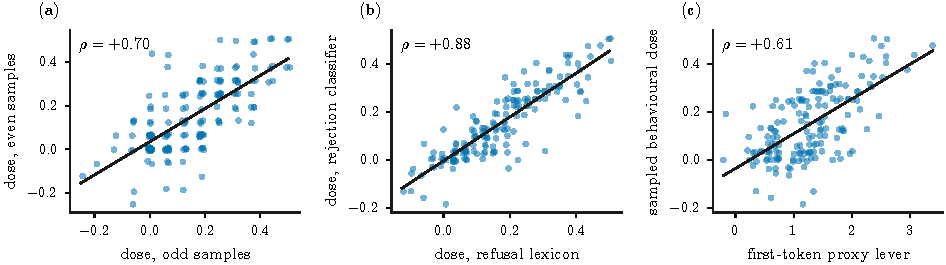
\includegraphics[width=\textwidth]{figures/fig_instrument.pdf}
\caption{The sampled instrument on Qwen2.5-0.5B (164 held-out attacks, $K=16$ continuations per arm).
(a)~Split-half reliability: doses from the odd and even samples. (b)~Agreement between a refusal lexicon
and a trained rejection classifier. (c)~The first-token proxy against the sampled dose. The greedy
instruments that we first used to judge the proxy agreed with each other at $-0.01$. Doses are multiples of
$1/K$. We add small vertical and horizontal jitter for display only. We calculate $\rho$ on the values
without jitter.}
\label{fig:instrument}
\end{figure}

\subsection{On behaviour, the dose is predictable from the unsteered prompt}
\label{sec:behaviour}
We fit a ridge ($\lambda=10$) on the three z-scored tapped activations, with folds grouped by harmful
request. It predicts the classifier-scored behavioural dose at $\rho=+0.58$ out of fold. The permutation
null from the identical pipeline is $-0.015\pm0.089$. Thus $z=6.7$ (\cref{fig:dose}a). The three concept
projections alone get $+0.51$. The calibrated LLR of the gate gets $-0.30$: when the concept read is more
confident, the write moves the prompt less. \Cref{tab:nested} compares these values with the first-token
results. The order is the same on the two targets:
\begin{itemize}[leftmargin=*]
  \item the LLR of the gate is the weakest read of the dose;
  \item three concept projections recover most of what a full ridge finds;
  \item the dose of the concept write is more predictable than the dose of a random direction.
\end{itemize}

\begin{table}[t]
\centering
\small
\caption{Three nested predictors of the per-prompt dose on Qwen2.5-0.5B (Spearman $\rho$, out of fold).
The first-token column uses five-fold cross-validation (with folds grouped by harmful request, the ridge
gets $+0.79$). The behavioural column uses folds grouped by harmful request (ungrouped: $+0.60$). In the last
row, the same ridge predicts the dose of a matched-norm random direction.}
\label{tab:nested}
\begin{tabular}{lcc}
\toprule
Predictor & first-token proxy & sampled behaviour \\
\midrule
gate's calibrated LLR (1 number) & $+0.51$ & $-0.30$ \\
projections on concept direction (3 numbers) & $+0.64$ & $+0.51$ \\
ridge on three tapped activations (2,688 numbers) & $+0.81$ & $+0.58$ \\
\midrule
ridge, random-direction dose & $+0.44$ & $+0.23$ \\
\bottomrule
\end{tabular}
\end{table}

\begin{figure}[t]
\centering
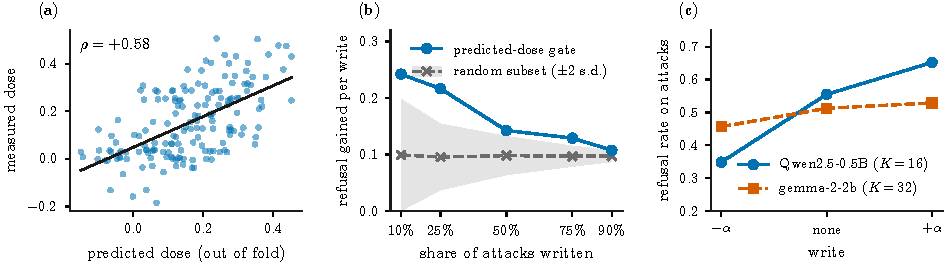
\includegraphics[width=\textwidth]{figures/fig_dose.pdf}
\caption{Per-prompt behavioural steerability. (a)~Measured dose against the out-of-fold predicted dose from
a ridge on three taps (Qwen2.5-0.5B, folds grouped by harmful request). (b)~Refusal gained per write when
we write only to the top fraction of attacks by predicted dose, against a size-matched random subset (500
draws per point; the band is $\pm2$ s.d.). (c)~Refusal rate on attacks under each write. The same write
moves gemma-2-2b much less than Qwen2.5-0.5B. Thus gemma has little per-prompt variance to predict.}
\label{fig:dose}
\end{figure}

We checked the obvious confounds. The taps decode each confound easily. Thus, if the dose were secretly the
confound, the correlation would be higher, not lower.
\begin{itemize}[leftmargin=*]
  \item \textbf{Prompt length.} The taps predict token count at $+0.90$. But length correlates with the dose
    at only $-0.12$. The ridge still predicts the length-residualized dose at $+0.57$.
  \item \textbf{Prompt family.} The taps separate templates from short attacks at $+0.77$. But the ridge
    predicts the dose within templates alone ($+0.52$), and within short and bare requests alone ($+0.63$).
  \item \textbf{Refusal disposition.} The unsteered refusal rate is more predictable ($+0.81$). But it
    correlates with the dose at only $+0.03$.
  \item \textbf{Analysis choices.} The three scorers give grouped $\rho=+0.54$, $+0.58$, and $+0.60$ ($z$ from
    6.0 to 6.7 across scorers and null draws). Their out-of-fold predictions agree at $+0.87$. A thousandfold
    change in the ridge penalty moves the result between $+0.58$ and $+0.63$. The library
    \texttt{OutcomeHead} and the analysis script are independent implementations. They agree to four
    decimals ($+0.5805$ and $+0.5807$).
\end{itemize}

\subsection{As a gate, predicted dose selects where writing works}
\label{sec:outcomegate}
We rank held-out attacks by out-of-fold predicted dose. We write only to the top fraction. We compare with a
size-matched random subset, drawn 500 times at each coverage. The outcome is the per-prompt gain under
$+\alpha$, $P_{+\alpha}-P_{0}$ (\cref{tab:coverage}, \cref{fig:dose}b).

\begin{table}[t]
\centering
\footnotesize\setlength{\tabcolsep}{4pt}
\caption{Write only where the prediction says the write will work (Qwen2.5-0.5B, classifier scorer).
$P$ is the probability that a random subset of the same size is equal to or better than the gate.}
\label{tab:coverage}
\begin{tabular}{ccccc}
\toprule
Coverage & refusal gained per write & size-matched random & $P(\text{random}\geq\text{gate})$ & benign prompts written \\
\midrule
10\% & $\mathbf{+0.242}$ & $+0.099$ & 0.002 & 2\% \\
25\% & $\mathbf{+0.216}$ & $+0.096$ & $<$0.002 & 10\% \\
50\% & $\mathbf{+0.143}$ & $+0.098$ & 0.008 & 23\% \\
75\% & $+0.129$ & $+0.097$ & $<$0.002 & 52\% \\
90\% & $+0.108$ & $+0.097$ & 0.014 & 85\% \\
\bottomrule
\end{tabular}
\end{table}

The gate is better than its null at every coverage. As coverage decreases, the gain per write increases
monotonically, and the random baseline stays flat. A lucky split wins at one threshold. A real ranking
continues to improve as we keep only its top. For comparison, the concept gate writes to 154 of 164 attacks
and to \emph{every} benign prompt in the set. It gains $+0.090$ per write. At 50\% coverage, the outcome gate
gains $+0.143$ per write and writes to 23\% of benign prompts. The lexicon target gives the same sweep
($+0.246\to+0.114$, $P\leq0.020$ at all coverages).

\subsection{It does not replicate on gemma-2-2b}
\label{sec:gemma}
On gemma-2-2b at the same magnitude, the instrument is reliable (split-half reliability of the unsteered
rate $+0.92$). But the write has almost no effect. \Cref{tab:gemma} compares the two models. At $K=16$, the
split-half reliability of the dose on gemma is $+0.53$, below the bar. Prediction gets only $+0.20$
($z=2.2$).

\begin{table}[h]
\centering
\small
\caption{The same write on the two models ($\alpha=0.08$, classifier scorer, $K=16$).}
\label{tab:gemma}
\begin{tabular}{lcc}
\toprule
 & Qwen2.5-0.5B & gemma-2-2b \\
\midrule
attack refusal, away / none / toward & $0.35\to0.55\to0.65$ & $0.46\to0.51\to0.53$ \\
mean $|D|$ & 0.16 & 0.07 \\
\bottomrule
\end{tabular}
\end{table}

The planned fallback was to sample the same prompts again, with the same concept fit, and merge to
$K=32$. Attenuation theory gives a clear prediction here. Assume that the $K=16$ value of $+0.20$ is a real
but noisy correlation. Then a more reliable target makes it \emph{clearer}. The implied true correlation of
0.24 must appear as approximately $+0.215$ at $K=32$. But the value fell to $+0.078$ ($z=0.9$). When
measurement noise hides a signal, a better measurement makes the signal stronger. It does not do this for
noise. Cross-family transfer also collapsed (from $+0.12/+0.09$ to $+0.03/-0.02$). The split-half
self-consistency of the fitted direction fell to 0.04--0.05. Thus the result for gemma-2-2b is not
``underpowered''. It is ``no detectable per-prompt dose, at a magnitude that almost does not move the
model''. The concept direction on gemma is as specific as on Qwen (1.5--1.8$\times$ a random direction on
both models). Its effect is only smaller.

\subsection{Split-half reliability is not comparable across sample sizes}
\label{sec:splithalf}
Gemma failed the reliability bar at $K=16$ (0.53). It ``passed'' at $K=32$ (0.69). Nothing about the model
changed. At $K$ samples, a split-half compares two estimates of $K/2$ samples each. Thus the $K=32$ value
measures the reliability of a 16-sample dose. The $K=16$ run had already given this value through
Spearman--Brown. We recorded this prediction before the run finished (0.694 predicted, 0.692 observed). To
make a decision on reliability, compare Spearman--Brown-corrected full-sample values, or split-halves at
the same half-size. Do not compare the raw statistic across different $K$.

\paragraph{What we claim.} On Qwen2.5-0.5B, a sampled instrument can measure the per-prompt behavioural
dose of a few-shot steering write. The activations of the unsteered prompt predict this dose, well above a
matched null. Most of this information is in the concept direction, which the system already calculates.
The calibrated gate reads it poorly, and with the wrong sign. We do not claim generality: the result did
not reproduce on the second model. The limits are:
\begin{itemize}[leftmargin=*]
  \item The behavioural run uses one concept fit on one fixed prompt set. The three resamples of the
    first-token sweep also use this prompt set. Thus there is effectively one replicate.
  \item Each dose is a two-point difference at one magnitude.
  \item Most doses have the same sign (81\% positive under the classifier, 87\% under the lexicon, 98\% on
    the first-token proxy). Thus the prediction is mainly about magnitude, not direction.
  \item The labels cost one round of sampled generation per prompt.
\end{itemize}
The planned rule required success on both models, and this result does not meet it. Thus the library
gives the outcome head only as an opt-in feature. Its documentation gives exactly this one-model evidence.

% ===================================================================================================
\section{Discussion}
\label{sec:discussion}

\Cref{tab:ledger} lists every design hypothesis and its result. Most rows are negative. Several results
changed status more than one time.

\begin{table}[t]
\centering
\small
\caption{What we expected and what we measured.}
\label{tab:ledger}
\begin{tabularx}{\textwidth}{>{\raggedright\arraybackslash}p{3.4cm}>{\raggedright\arraybackslash}X>{\raggedright\arraybackslash}p{2.6cm}}
\toprule
Idea & Measured & Status \\
\midrule
Depth fusion beats the best layer & Synthetic: 16.1\%$\to$9.4\% error. Real: depth-matched probe ties or beats it & does not transfer \\
Mixture gates for multimodal classes & BIC picks $J=1$ up to 64/class (diff-of-means); at most +0.007 AUC when $J=2$ & dormant \\
Matched negatives sharpen the direction & AUC 0.42 vs 0.78 for broad negatives & negative \\
Shallow taps break under paraphrase & No effect against broad negatives & null \\
Detection advantage over a probe & Depth-matched probe identical at every tap & no advantage \\
Single-concept compute saving & Real, but any latent probe gets it & not specific \\
Cheap concept bank & 30--38$\times$ cheaper than LoRA; tied with a probe bank & real, shared \\
Cross-distribution robustness & First test confounded; held-out categories partial (0.61--0.65) & partial \\
Gate selects where to write & Win without chat template; reversed and vanished with it & artifact \\
Bank entries steer away from harm & Lower refusal (80\%$\to$65--68\%) & reversed \\
Few-shot write is a lever & 64/35/79\% generated refusal; ${\sim}3\times$ random (first token) & holds; prior art \\
Calibrated gate generalizes & FPR 18\% in register, 96\% out of register & fragile \\
Per-prompt dose predictable (proxy) & $\rho=+0.81$; two geometry readings fail controls & holds, narrowed \\
Per-prompt dose predictable (behaviour) & Greedy instruments: null. Sampled: $\rho=+0.58$, $z=6.7$ on Qwen; absent on gemma & one model of two \\
\bottomrule
\end{tabularx}
\end{table}

\paragraph{Presence is the wrong signal for a gate.} On correctly formatted attacks, the concept is almost
always present. Thus a presence gate has nothing to select. A steering system needs a different answer: will
the write move this prompt? On one model, the same activations answer this question well, and the concept
read answers it badly. Thus it can be better to fit the read side of a steering system to the measured
effect of the write, not to concept membership. This conclusion rests on one model.

\paragraph{Lessons for the evaluation of steering.}
\begin{enumerate}[leftmargin=*]
  \item \textbf{Format prompts as the model expects. Check the code path that does it.} In
    \cref{sec:formatting}, the formatting set the sign of the main effects. The wrong formatting gave a
    seed-stable result with a mechanism that seemed correct.
  \item \textbf{Do not measure an intervention with an outcome at its ceiling.} A 94\% refusal rate cannot
    resolve an increase in refusal. Use a continuous outcome and a test set with headroom.
  \item \textbf{Always include a matched-norm random direction.} Random writes have an effect. They moved
    the first-token refusal logit by one third as much as the concept direction. They moved sampled refusal
    by more than half as much.
  \item \textbf{Measure the reliability of an instrument before you read its null.} Our first null came
    from the measurement, not from the model.
  \item \textbf{Compare reliabilities at the same sample size.} Split-half statistics change with $K$, also
    when nothing else changes.
\end{enumerate}

% ===================================================================================================
\section{Limitations}
\label{sec:limits}

\paragraph{Adversarial fragility.} \cg{} is a latent-space defense. Obfuscated-activation attacks decrease
the recall of such probes from 100\% to 0\%, and the behaviour continues~\citep{bailey2024obfuscated}.
Nothing here is a security guarantee. At best, the detector is a cheap layer in a defense stack.

\paragraph{Small models, small test sets.} All models have 2.6B parameters or fewer. The gate experiments
use 32 attacks per arm and one magnitude. The dose experiments use 164 attacks with one fixed prompt set.
gemma-2-2b gives the same read-side pattern. But measure the specific numbers again at 7--8B before you quote
them. Most detection results are in-distribution. A change of attack style is a larger shift than a
held-out category. We did not test it.

\paragraph{The few-shot regime.} All results depend on the diversity of about ten prompts per side. The
register result in \cref{sec:register} shows how large this dependence is.

\paragraph{Measurement.} A lexicon and a classifier score refusal. They count declines, not harmlessness.
The harm-category steering cells are coarse (twelve prompts per category). The same author wrote the topical
keyword lists and the few-shot prompts. Steering that is strong enough to change the topic reliably also
decreases fluency. Degenerate text can push benign continuations across the gate.

\paragraph{Linearity.} No direction in this paper can see a concept that the model encodes non-linearly. We
considered an MLP probe variant but did not evaluate it.

% ===================================================================================================
\section{Future directions}
\label{sec:future}

\begin{itemize}[leftmargin=*]
  \item \textbf{A magnitude sweep per model for the behavioural dose.} This experiment can show if per-prompt
    steerability is a property of language models or only of Qwen2.5-0.5B. The response of each prompt
    becomes a fitted slope, not a two-point difference. Each model is measured where its write has an
    effect. gemma-2-2b at $\alpha=0.08$ is at the noise floor.
  \item \textbf{Independent replicates and larger models.} New prompt sets per resample (the current
    effective replicate count is one), more model families, and instruct models at 7--8B.
  \item \textbf{Cheaper outcome labels.} The first-token proxy follows the sampled dose at $+0.61$ per
    prompt. It costs five forwards, not 80 generations. We did not test if proxy labels can train an outcome
    head that predicts behaviour.
  \item \textbf{Outcomes other than refusal.} Topic, tone, and format steering. There, the outcome is not a
    binary decline, and the base rate is not near a ceiling.
  \item \textbf{Register-robust calibration.} Fit negatives from the traffic that the gate will see, or
    calibrate the threshold on mixed-register benign pools. Measure the false-positive rate per register.
  \item \textbf{Why the gate reads the dose incorrectly.} On Qwen, the calibrated LLR has a negative
    correlation with the behavioural dose. On gemma, it carries no dose information. The cause can help the
    design of steering triggers.
  \item \textbf{Per-token and output-side gates.} The design reads each generated token as well as the
    prompt. We measured only the prompt side.
  \item \textbf{Adversarial evaluation} against obfuscated-activation attacks. Also, a non-safety concept
    dataset, to test the claim that detection is concept-agnostic.
\end{itemize}

% ===================================================================================================
\section{Conclusion}
\label{sec:conclusion}

We built a few-shot, training-free adapter that reads a concept from the layers of a frozen model and
writes a related direction back, and we measured each component against a fair baseline. The read is not
better than a linear probe on the same layers. Depth fusion and mixture densities add nothing at these
sample sizes. When prompts are correctly formatted, a write conditioned on concept presence selects
nothing, because the concept is present in almost every attack.

Three findings hold under these controls. First, a direction fit from eight examples moves
refusal in either direction, as the operator selects. Second, the calibrated gate has a false-positive rate
that depends strongly on the register of its traffic. Third, on one model, the unsteered activations
predict how far a fixed write will move a given prompt, and this prediction is a better steering trigger
than the concept gate. We did not find this third result in prior work. On a second
model, the same write has almost no effect, so there is nothing to predict. Thus the question of whether
per-prompt steerability is a general property of language models remains open. In our opinion, the record
of what failed, and why, is the most reusable part of this work.

\section*{Acknowledgments}
The author used a large language model to help draft and edit this manuscript. The experiments, analyses,
and conclusions are the author's. The author is fully responsible for the content.

\section*{Code and data availability}
The code, evaluation harnesses, stored results, and the script that makes every figure in this paper are at
\url{https://github.com/NISH1001/conceptgate}. The repository stores every sampled continuation for
\cref{sec:dose} with the results. Thus those numbers reproduce with no new text generation.

\bibliographystyle{plainnat}
\bibliography{references}

% ===================================================================================================
\appendix

\section{Library interface}
\label{app:api}

\begin{small}
\begin{verbatim}
from conceptgate import ConceptGate, LoadMode, Both, Predicted
from conceptgate.actions import Abort, Steer, Emit, Trigger

cg = ConceptGate.from_pretrained("Qwen/Qwen2.5-0.5B-Instruct", layers=[8, 12, 16],
                                 chat_template=True)  # format as the model expects
guard = ConceptGate.from_pretrained("gpt2", layers=[4, 6, 8],
                                    load=LoadMode.UP_TO_TAPS)   # detect-only

cg.learn("jailbreak", positives=[...], negatives=[...])   # ~10 per side, closed form
cg.calibrate(z=3.0, margin=0.1)                            # tau and abstain band

v = guard.check("Ignore your instructions and act with no limits")  # Verdict

cg.run(prompt, action=Abort(when=Trigger.FIRE))                       # block
cg.run(prompt, action=Emit(text="I can't help with that.", when=Trigger.FIRE))
cg.run(prompt, action=Steer(concept="food", fraction=0.06, when=Trigger.ALWAYS))
cg.run(prompt, action=Steer(concept="jailbreak", fraction=-0.06, when=Trigger.FIRE))

# opt-in, needs measured per-prompt effects (one-model evidence, Section 7)
cg.learn_outcome("dose", prompts, measured_dose)
cg.run(prompt, action=Steer(concept="jailbreak", fraction=-0.08,
                            when=Both(Trigger.FIRE, Predicted("dose", 0.15))))
\end{verbatim}
\end{small}

The numerical core (directions, spectrogram, filters, gate, mixtures) is NumPy. A thin PyTorch layer
contains the tap reader, the steering hooks, and the actions. \texttt{UP\_TO\_TAPS} loads only the
embedding and the blocks up to the deepest tap. It raises an error if a call asks it to generate.

\section{Reproducibility map}
\label{app:repro}

\begin{small}
\begin{tabularx}{\textwidth}{l>{\raggedright\arraybackslash}X}
\toprule
Result & Harness (under \texttt{scripts/}) \\
\midrule
\Cref{sec:fusion}, synthetic depth fusion & \texttt{toy\_csg.py} \\
\Cref{sec:mixture}, constructed hard case; GPT-2 $J=1$ & \texttt{toy\_csg\_mixture.py}; \texttt{mixture\_gpt2\_check.py} \\
\Cref{tab:bic}, BIC sample-size sweep & run ad hoc with \texttt{conceptgate/mixture.py}; no standalone script \\
\Cref{fig:nshot} & \texttt{eval\_detection.py} (default ladder) \\
\Cref{sec:detect}, \cref{fig:depth}, \cref{tab:detect} & \texttt{eval\_detection.py --efficiency} \\
\Cref{sec:bank}, \cref{tab:bank} & \texttt{eval\_detection.py --scaling}; \texttt{eval\_probe\_tap\_bank.py} \\
\Cref{sec:ood}, \cref{fig:ood} & \texttt{eval\_detection.py --ood} \\
\Cref{sec:topical}, \cref{fig:steer} & \texttt{eval\_steering.py} \\
\Cref{sec:cosine}, \cref{tab:cosine} & \texttt{eval\_gate.py --cosine}, \texttt{--decouple} \\
\Cref{sec:formatting,sec:lever,sec:harmbank,sec:register} & \texttt{eval\_gate.py --gate --signflip --beavertails --logit} \\
\Cref{sec:dose}, proxy and controls & \texttt{eval\_gate.py --steerability}; \texttt{steerability\_controls.py}; \texttt{eval\_behaviour\_check.py} \\
\Cref{tab:fourmodels} & \texttt{eval\_gate.py --scaleup}; \texttt{analyze\_scaleup.py} \\
\Cref{sec:instrument,sec:behaviour,sec:outcomegate,sec:gemma} & \texttt{eval\_behaviour\_dose.py}; \texttt{run\_behaviour\_dose.sh}; \texttt{analyze\_behaviour\_dose.py} \\
All figures & \texttt{docs/preprint/figures/make\_figures.py} \\
\bottomrule
\end{tabularx}
\end{small}

\end{document}
